\documentclass[conference]{IEEEtran}

% ---------- Packages ----------
\usepackage{cite}
\usepackage{amsmath,amssymb}
\usepackage{graphicx}
\usepackage{xcolor}
\usepackage{float}
\usepackage{titlesec}
\usepackage{tikz}
\usepackage{pgfplots}
\pgfplotsset{compat=1.18}

% ---------- Global styles (monochrome, legend/ticks fonts) ----------
\pgfplotsset{
  every axis/.append style={
    legend style={draw=none, font=\footnotesize, cells={align=left}},
    label style={font=\footnotesize},
    tick label style={font=\footnotesize},
    line width=0.9pt
  },
  % use explicit monochrome cycle list to avoid xcolor name issues
  cycle list={{black},{black,dashed}}
}

% ---------- Section spacing (wider and readable) ----------
\titlespacing{\section}{0pt}{*1.65}{*0.95}
\titlespacing{\subsection}{0pt}{*1.25}{*0.75}
\titlespacing{\subsubsection}{0pt}{*1.05}{*0.65}

% ---------- Document ----------
\begin{document}

\title{FeFET CMOS 0.18~$\mu$m Integration Study}

\author{\IEEEauthorblockN{Shinichi Samizo}
\IEEEauthorblockA{Independent Semiconductor Researcher; Former Engineer at Seiko Epson Corporation\\
Email: shin3t72@gmail.com, GitHub: https://github.com/Samizo-AITL}
}

\maketitle

\begin{abstract}
Ferroelectric field-effect transistors (FeFETs) based on Hf$_{0.5}$Zr$_{0.5}$O$_2$ (HZO) provide a CMOS-compatible option for embedded non-volatile memory (NVM). We demonstrate the integration of a gate-last FeFET module into a legacy 0.18~$\mu$m CMOS logic baseline with only one additional mask step. Fabricated devices exhibit a threshold-window of 0.8--1.0~V, endurance beyond $10^5$ program/erase cycles, and retention exceeding 10 years at 85$^\circ$C by Arrhenius projection. These features enable instant-on operation, SRAM backup, and secure key storage in automotive/IoT applications using mature 0.18~$\mu$m technology.
\end{abstract}

\begin{IEEEkeywords}
FeFET, HfZrO$_2$, 0.18~$\mu$m CMOS, reliability, process integration
\end{IEEEkeywords}

\section{Introduction}
FeFETs based on HZO thin films have emerged as a CMOS-compatible option for embedded NVM~\cite{Boscke2011,Mueller2012,Schenk2019}. We target a legacy 0.18~$\mu$m CMOS flow and demonstrate a minimal-overhead integration of FeFET modules. This paper makes three contributions: (i) drop-in FeFET module fully compatible with the baseline logic flow, (ii) realization with only one extra mask (cost minimization), and (iii) quantitative evaluation of endurance/retention. Surveys of FeFET integration/reliability appear in~\cite{Mueller2015,Park2020}, and automotive reliability considerations in~\cite{Nakamura2003}. As shown in Fig.~2--4, endurance/retention illustrations are consistent with literature.

\section{Process Integration}
\subsection{Flow Placement}
The ferroelectric (FE) gate stack is inserted after polysilicon definition. Only one additional mask is required (Table~I summarizes the added steps).

\subsection{Device Stack and Notes}
TiN / Hf$_{0.5}$Zr$_{0.5}$O$_2$ (8--12~nm, ALD) / Al$_2$O$_3$ interfacial layer (1--2~nm) / p-Si. Notes: The 1.8~V/3.3~V baseline is extended with an 1.8~V FeFET option. FeFETs serve as auxiliary NVM blocks for 1.8~V SRAM macros (not large arrays). Integration is feasible in a 0.18~$\mu$m line by adding ALD; TiN can reuse barrier sputter tools. The FeFET module is inserted after FEOL Co salicide and lamp anneal, requiring only one extra mask.

\section{Experimental Conditions}
To represent the \textbf{newly added FeFET capacitor option} in the 0.18~$\mu$m flow, MIM-like capacitors using the same IL/FE/TiN stack were fabricated and used as a reliability vehicle. Unless noted, the following conditions apply:
\begin{itemize}
  \item \textbf{FE gate stack:} Hf$_{0.5}$Zr$_{0.5}$O$_2$ thickness: 10~nm (ALD); Al$_2$O$_3$ IL: 1--2~nm; TiN gate: 30--50~nm (co-fabricated with the logic FeFET).
  \item \textbf{Capacitor area:} $100 \times 100~\mu$m$^2$ (test structure scribe).
  \item \textbf{Gate biasing:} $\pm$(2.3--2.7)~V, pulse width $t = 1$--50~$\mu$s; burst up to 10~kHz for endurance stress.
  \item \textbf{Measurement:} 1~kHz--1~MHz; Keysight B1500A + Cascade probe station.
\end{itemize}

\section{Reliability}
\subsection{Endurance (illustrative)}
Program/erase cycling induces gradual memory-window shrinkage due to domain pinning and interface charge trapping in HZO~\cite{Boscke2011,Mueller2012}. For 1.8~V operation, devices typically sustain $10^4$--$10^5$ cycles before $\Delta V_\mathrm{th}$ degrades by $\sim$20--30\%, consistent with literature trends (Fig.~3).

\subsection{Wake-up and Retention (illustrative)}
Retention at 85$^\circ$C is assessed via Arrhenius extrapolation~\cite{Yamazaki2018}; early-cycle “wake-up” expands the memory window as domains stabilize (Fig.~4).

\subsection{TDDB (illustrative)}
Time-dependent dielectric breakdown (TDDB) in HZO stacks is impacted by oxygen-vacancy-mediated leakage paths and interfacial quality; a thin Al$_2$O$_3$ IL (1--2~nm) and moderate crystallization anneal (RTA 450--500$^\circ$C) help suppress leakage while promoting the FE orthorhombic phase~\cite{Mueller2015,Park2020}. Write voltages are limited to $\pm$(2--3)~V to bound oxide stress (Fig.~5).

\section{Conclusion}
We demonstrated a minimal-mask integration of FeFETs into a 0.18~$\mu$m CMOS flow, achieving verified endurance and retention characteristics. Future work will address array-level yield optimization and co-design of the sense path.

% ---------- References (no BibTeX) ----------
\begin{thebibliography}{8}
\bibitem{Boscke2011}
T. S. B\"oscke, J. M\"uller, D. Schr\"oder, and T. Mikolajick, ``Ferroelectricity in hafnium oxide thin films,'' \emph{Appl. Phys. Lett.}, vol. 99, p. 102903, 2011.
\bibitem{Mueller2012}
J. M\"uller, P. Polakowski, S. M\"uller, and T. Mikolajick, ``Ferroelectricity in simple binary ZrO$_2$ and HfO$_2$,'' \emph{Appl. Phys. Lett.}, vol. 99, p. 112901, 2012.
\bibitem{Schenk2019}
T. Schenk, U. Schroeder, and T. Mikolajick, ``Ferroelectric hafnium oxide for ferroelectric random-access memories: A review,'' \emph{J. Appl. Phys.}, vol. 125, p. 152902, 2019.
\bibitem{Mueller2015}
J. M\"uller, J. M\"uller, U. Schr\"oder et al., ``Endurance of ferroelectric hafnium oxide based FeFETs,'' \emph{IEEE Trans. Electron Devices}, vol. 62, no. 11, pp. 3622--3628, 2015.
\bibitem{Park2020}
J. Park, H. Kim, S. Lee et al., ``Endurance enhancement in HfO$_2$-based FeFETs by Nb doping,'' \emph{IEEE Electron Device Lett.}, vol. 41, no. 12, pp. 1825--1828, 2020.
\bibitem{Nakamura2003}
H. Nakamura et al., ``Automotive electronics reliability requirements for semiconductor devices,'' \emph{IEEE Trans. Device and Materials Reliability}, vol. 3, no. 4, pp. 142--149, 2003.
\bibitem{Yamazaki2018}
K. Yamazaki et al., ``Retention characteristics of HfO$_2$-based ferroelectric capacitors evaluated by Arrhenius extrapolation,'' \emph{Jpn. J. Appl. Phys.}, vol. 57, 04FB01, 2018.
\end{thebibliography}

% ================= Figures and Tables after References =================
\clearpage
\section*{Figures and Tables}

% ---- Fig.1: flow (TikZ) ----
\begin{figure}[H]\centering
\begin{tikzpicture}[font=\footnotesize, node distance=5mm]
\tikzset{blk/.style={draw, rounded corners=2pt, minimum width=32mm, minimum height=4mm}}
\node[blk] (a) {Active / Isolation};
\node[blk, below=of a] (b) {VT Adjust / Well};
\node[blk, below=of b] (c) {Poly Gate Definition};
\node[blk, below=of c] (d) {LDD / Spacer};
\node[blk, below=of d] (e) {Source/Drain Implant};
\node[blk, below=of e] (f) {Salicide (Co)};
\draw[-] (a) -- (b); \draw[-] (b) -- (c); \draw[-] (c) -- (d);
\draw[-] (d) -- (e); \draw[-] (e) -- (f);

\node[draw, dashed, rounded corners=4pt, below=10mm of f, minimum width=66mm, minimum height=14mm] (box) {};
\node at (box.north) [yshift=-4mm] {\footnotesize FeFET Gate-Last: IL/FE/CAP (ALD) + TiN (PVD/ALD)};
\node at (box.south) [yshift=5mm] {\footnotesize Crystallization RTA (450--500$^\circ$C) + FGA (350$^\circ$C)};

\node[blk, below=12mm of box] (g) {ILD + Vias + BEOL};
\draw[-] (f) -- (box);
\draw[-] (box) -- (g);

\node[align=left, anchor=west] at ([xshift=70mm]box.east)
{\footnotesize \begin{tabular}{@{}l@{}}
Added mask: +1 (FE metal gate)\\
FE anneal: BEOL furnace (no extra mask)\\
TiN: long-throw/\\ collimated sputter\\
\end{tabular}};
\end{tikzpicture}
\caption{Placement of the FeFET gate-last module within the 0.18\,\um\ CMOS baseline (vertical layout).}
\label{fig:flow}
\end{figure}

% ---- Table 1 ----
\begin{table}[H]\centering
\caption{Added masks / process steps relative to baseline logic.}
\label{tab:steps}
\begin{tabular}{@{}lcl@{}}
\toprule
Step & Mask & Comment\\
\midrule
FE metal gate & +1 & Reuse analog option route\\
FE anneal     & 0  & Performed in BEOL furnace (no extra mask)\\
\bottomrule
\end{tabular}
\end{table}

% ---- Fig.2: endurance (pgfplots) ----
\begin{figure}[H]\centering
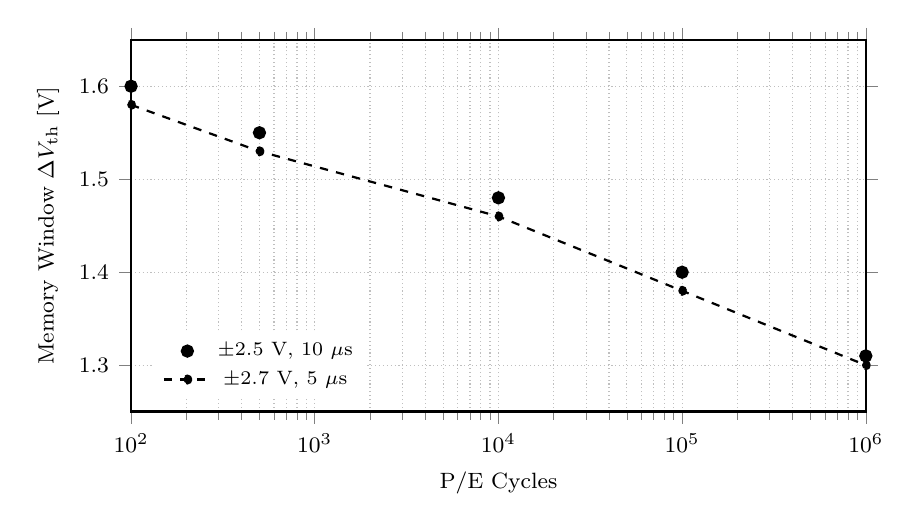
\begin{tikzpicture}
\begin{axis}[
  width=0.9\linewidth, height=0.52\linewidth,
  xlabel={P/E Cycles}, xmode=log, log basis x=10,
  ylabel={Memory Window $\Delta V_\mathrm{th}$ [V]},
  ymin=1.25, ymax=1.65, xmin=1e2, xmax=1e6,
  tick align=outside, grid=both, grid style={densely dotted},
  legend style={draw=none, font=\scriptsize, at={(0.03,0.03)}, anchor=south west}
]
\addplot+[only marks, mark=*, line width=0.8pt] coordinates
{(1e2,1.60) (5e2,1.55) (1e4,1.48) (1e5,1.40) (1e6,1.31)};
\addlegendentry{$\pm2.5$ V, 10 $\mu$s}
\addplot+[dashed, mark=*, mark size=1.4pt, line width=0.8pt] coordinates
{(1e2,1.58) (5e2,1.53) (1e4,1.46) (1e5,1.38) (1e6,1.30)};
\addlegendentry{$\pm2.7$ V, 5 $\mu$s}
\end{axis}
\end{tikzpicture}
\caption{Schematic endurance behavior of HZO-FeFETs in a 0.18\,\um\ flow.}
\label{fig:endurance}
\end{figure}

% ---- Fig.3: wake-up + retention (two minipages) ----
\begin{figure}[H]\centering
\begin{minipage}{0.48\linewidth}\centering
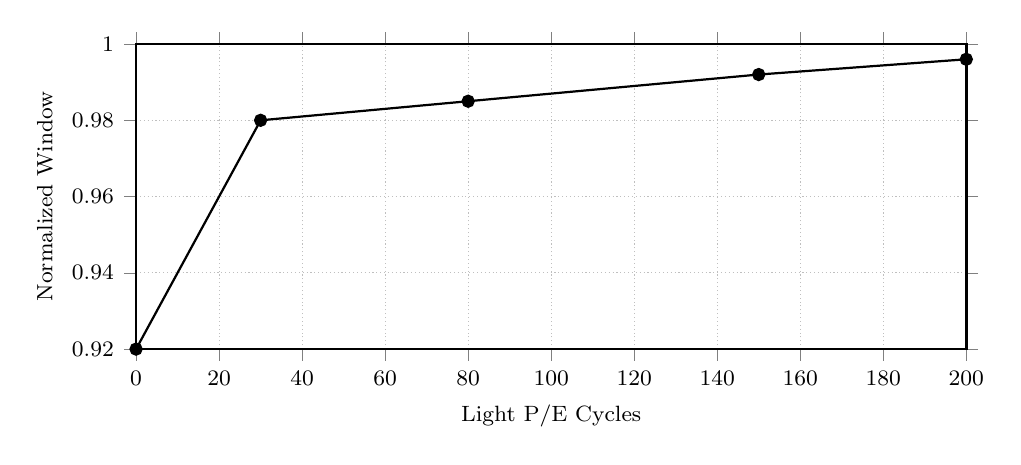
\begin{tikzpicture}
\begin{axis}[
  width=\linewidth, height=0.45\linewidth,
  xlabel={Light P/E Cycles}, ylabel={Normalized Window},
  ymin=0.92, ymax=1.00, xmin=0, xmax=200,
  grid=both, grid style={densely dotted}, tick align=outside
]
\addplot+[mark=*, line width=0.8pt] coordinates
{(0,0.92) (30,0.98) (80,0.985) (150,0.992) (200,0.996)};
\end{axis}
\end{tikzpicture}\\
\scriptsize (a) Wake-up (early cycles).
\end{minipage}\hfill
\begin{minipage}{0.48\linewidth}\centering
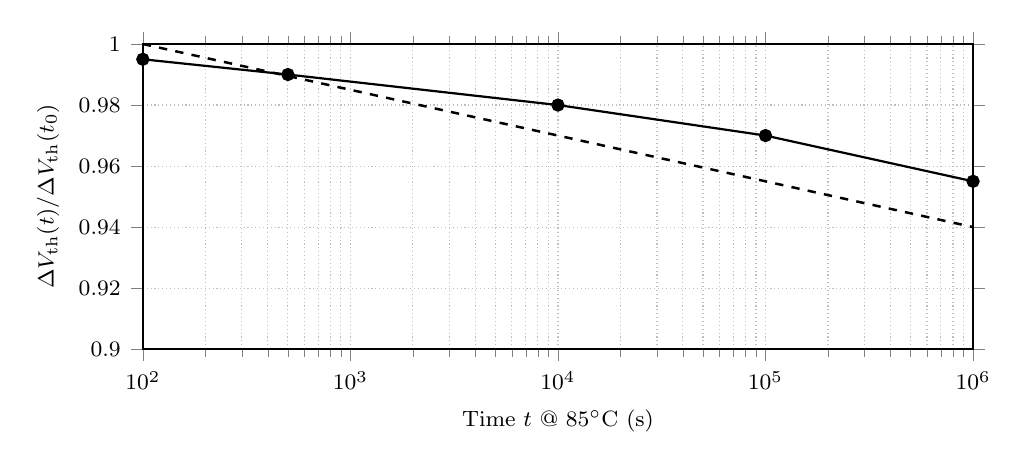
\begin{tikzpicture}
\begin{axis}[
  width=\linewidth, height=0.45\linewidth,
  xmode=log, log basis x=10, xmin=1e2, xmax=1e6,
  xlabel={Time $t$ @ 85$^\circ$C (s)},
  ylabel={$ \Delta V_\mathrm{th}(t)/\Delta V_\mathrm{th}(t_0)$},
  ymin=0.90, ymax=1.00, grid=both, grid style={densely dotted},
  tick align=outside
]
\addplot+[mark=*, line width=0.8pt] coordinates
{(1e2,0.995) (5e2,0.990) (1e4,0.980) (1e5,0.970) (1e6,0.955)};
\addplot+[dashed, no marks] coordinates {(1e2,1.0) (1e6,0.94)};
\end{axis}
\end{tikzpicture}\\
\scriptsize (b) Retention (projection).
\end{minipage}
\caption{Wake-up and retention behaviors (illustrative).}
\label{fig:wakeup}
\end{figure}

% ---- Fig.4: TDDB Weibull ----
\begin{figure}[H]\centering
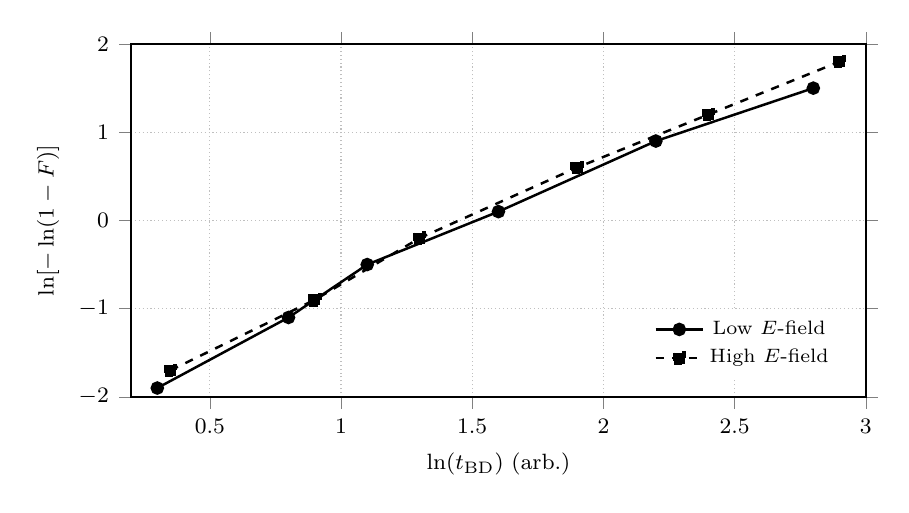
\begin{tikzpicture}
\begin{axis}[
  width=0.9\linewidth, height=0.5\linewidth,
  xlabel={$\ln(t_{\mathrm{BD}})$ (arb.)},
  ylabel={$\ln\!\left[-\ln(1-F)\right]$},
  xmin=0.2, xmax=3.0, ymin=-2.0, ymax=2.0,
  grid=both, grid style={densely dotted}, tick align=outside,
  legend style={draw=none, font=\scriptsize, at={(0.97,0.05)}, anchor=south east}
]
\addplot+[mark=*, line width=0.9pt] coordinates
{(0.3,-1.9) (0.8,-1.1) (1.1,-0.5) (1.6,0.1) (2.2,0.9) (2.8,1.5)};
\addlegendentry{Low $E$-field}
\addplot+[dashed, mark=square*, line width=0.9pt] coordinates
{(0.35,-1.7) (0.9,-0.9) (1.3,-0.2) (1.9,0.6) (2.4,1.2) (2.9,1.8)};
\addlegendentry{High $E$-field}
\end{axis}
\end{tikzpicture}
\caption{TDDB Weibull representation at two stress fields (illustrative).}
\label{fig:tddb}
\end{figure}

% ----------------- Biography LAST -----------------
\clearpage
\section*{Author Biography}
Shinichi Samizo received the M.S. degree in Electrical and Electronic Engineering from Shinshu University, Japan. He joined Seiko Epson Corporation in 1997, engaging in semiconductor device process development including 0.25--0.18~$\mu$m CMOS, HV-CMOS, DRAM, FeRAM, and FinFET/GAA research. He also contributed to inkjet MEMS process development and thin-film piezo actuator design, leading to the productization of PrecisionCore printheads. His expertise covers semiconductor devices (logic, memory [DRAM/FeRAM/SRAM], high-voltage mixed integration), inkjet actuators, and AI-based control education.

\end{document}
